\documentclass[handout]{beamer}
 
\usepackage[utf8]{inputenc}
\usepackage{mathtools}
\usepackage{tikz}

\usetheme{CambridgeUS}
% \useoutertheme{split}
\setbeamertemplate{title page}[default][colsep=-4bp,rounded=true]

% only inlcude the current secition in the header
\AtBeginSection{
    \begin{frame}
        \tableofcontents[sections=\value{section}, sectionstyle=show/show]
    \end{frame}
}

\usetikzlibrary{calc,shapes}
\usetikzlibrary{fit,positioning,decorations.pathreplacing,calligraphy}

\tikzstyle{key}=[circle, thin, minimum width=\ln, minimum height=\hn, draw=black, fill=white, inner sep=0cm, anchor=north]
\tikzstyle{fts}=[key,fill=gray!50,minimum width=0.8*\ln]
\tikzstyle{hash}=[key,rectangle, anchor=north]

\renewcommand{\ln}{6mm} % largeur de noeud
\newcommand{\hn}{6mm}    % hauteur de noeud
\renewcommand{\le}{5mm} % largeur de l'espace
\newcommand{\he}{8mm}   % hauteur de l'espace

\newcommand{\hasharrow}[2]{ \draw (H#2.north) -- ($(H#2.north)+(0,.5*\he)$) -- ($(H#1.south)+(0,-.5*\he)$) -> (H#1.south); }
\newcommand{\keyhasharrow}[2]{ \draw (K#2.north) -- ($(K#2.north)+(0,.5*\he)$) -- ($(H#1.south)+(0,-.5*\he)$) -> (H#1.south); }
\newcommand{\signarrow}[2]{ \draw (K#1.south) edge[dashed,->] (H#2.north); }


%Information to be included in the title page:
\title{Zero Knowledge}
\author{Rohit Musti}
\institute{CUNY - Hunter College}
\date{\today}
 
\begin{document}
 
\frame{\titlepage}

\section{Overview}

\begin{frame}{Intuition}
    \begin{itemize}
        \item \pause How can we prove a statement \(x\) is true without revealing anything other than that statement is true (without resorting to a trusted actor)?
        \item \pause How can we prove we know where Waldo is in a Where's waldo game without revealing Waldo's location?
        \item \pause How do we prove a child is tall enough to ride a ride at an amusement park without revealing the child's true height, hair color, etc.?
        \item \pause How can we approve you can afford to buy a coffee without revealing your networth, bank account total, preferred currency, etc.?
        \item \pause How can we prove \(N\) is the product of two primes \(p, q\) without revealing its factorization?
    \end{itemize}
\end{frame}

\begin{frame}{Definitions}
    \begin{itemize}
        \item \pause What is knowledge? In cryptography, we refer to knowledge as things that can be computed efficiently. \pause If you know \(N\), \(p\), you \textit{know} \(q\).
        \item \pause It follows that a zero knowledge protocol is a protocol that doesn't reveal any information that the adversary could not otherwise efficiently compute. 
        \item \pause If you had a protocol that proved you knew the \(m\) that a \(c\) encrypted, you wouldn't reveal any information that an adversary could easily compute from \(c\) directly
    \end{itemize}
\end{frame}

\section{Examples}

\begin{frame}{Ali Baba Cave}
    \begin{itemize}
        \item \pause Our two friends and protagonists, Alice and Bob, are on an adventure and stumble onto a Cave
        \item \pause There are two different entrances to two different paths and there is a door somewhere in the cave connecting the two paths!
        \item \pause Alice knows this door's code and offers to sell it to Bob! However, Bob wants proof that the code works and Alice refuses to reveal the code without Bob purchasing it!
        \item \pause Bob offers to follow Alice into the cave and then close his eyes while Alice taps in the code, but it is dark in the cave and Alice has no way to be sure that Bob actually has his eyes closed!
    \end{itemize}
\end{frame}

\begin{frame}{Ali Baba Cave}
    \begin{itemize}
        \item \pause Our two friends are at an impasse, but then their hip friend Suhail wanders by fresh from his Introduction to Cryptography lecture and offers this solution! 
        \item \pause Suhail suggests that Alice picks any one of the paths to enter into the cave. Then, then Bob can call out which path he wants Alice to exit from.
        \item \pause There is a 50\% chance that Alice and Bob select the same path. However, over multiple runs, it is unlikely that they repeatedly choose the same path
    \end{itemize}
\end{frame}

\begin{frame}{Discrete Log}
    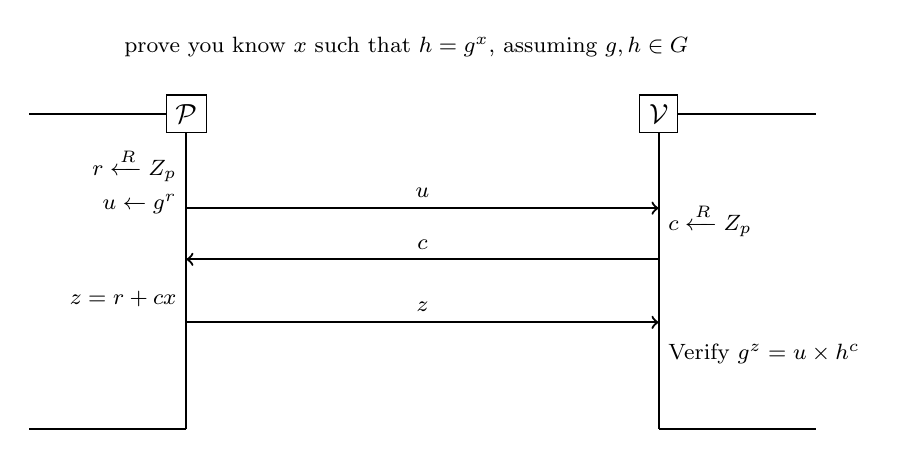
\begin{tikzpicture}
      \pause
        \node[draw] (Adversary) at (-3, 2) {\(\mathcal{P}\)}; 
        \draw[thick] (Adversary) -- ++(0, -4); 
        \draw[thick] (Adversary) -- ++(-2, 0);
        \draw[thick] (-3, -2) -- ++(-2, 0);

      \pause
        \node[draw] (Challenger) at (3,2) {\(\mathcal{V}\)}; 
        \draw[thick] (Challenger) -- ++(0, -4);
        \draw[thick] (Challenger) -- ++(2, 0);
        \draw[thick] (3, -2) -- ++(2, 0);

      \pause
        \node[draw=none,fill=none,anchor=east, font=\footnotesize] (choice0) at ($(Adversary) + (6.5,.85)$) {prove you know \(x\) such that \(h = g^x\), assuming \(g, h \in \mathbb{G}\)};

      \pause
        \node[draw=none,fill=none,anchor=east, font=\footnotesize] (choice0) at ($(Adversary) + (0,-.65)$) {\(r \xleftarrow[]{R} \mathbb{Z}_{p}\)};
        \node[draw=none,fill=none,anchor=east, font=\footnotesize] (choice0) at ($(Adversary) + (0,-1.15)$) {\(u \leftarrow g^{r}\)};
      \pause
        \draw[->,thick] ($(Adversary)+(0,-1.2)$) -- ($(Challenger)+(0,-1.2)$) node [pos=0.5,above,font=\footnotesize] {\(u\)};
      \pause
        \node[draw=none,fill=none,anchor=west, font=\footnotesize] (bit) at ($(Challenger) + (0,-1.35)$) {\(c \xleftarrow[]{R} \mathbb{Z}_{p}\)};
      \pause
        \draw[->,thick] ($(Challenger)+(0,-1.85)$) -- ($(Adversary)+(0,-1.85)$) node [pos=0.5,above,font=\footnotesize] {\(c \)};
      \pause 
        \node[draw=none,fill=none,anchor=east, font=\footnotesize] (choice0) at ($(Adversary) + (0,-2.35)$) {\(z = r + cx\)};
      \pause
        \draw[->,thick] ($(Adversary)+(0,-2.65)$) -- ($(Challenger)+(0,-2.65)$) node [pos=0.5,above,font=\footnotesize] {\(z\)};
      \pause
        \node[draw=none,fill=none,anchor=west, font=\footnotesize] (bit) at ($(Challenger) + (0,-3.05)$) {Verify \(g^z = u \times h^c\)};
      \end{tikzpicture}
\end{frame}

\begin{frame}{Discrete Log ZK Authentication Protocol}
    \begin{itemize}
        \item \pause What if an adversary has hacked the server and can see clients interaction with the server!
        \item \pause Non-Zero Knowledge protocols will lead to compromise identities for people who try and log in.
        \item \pause If the server stores \(g, g^x\) and the server and client complete the zero-knowledge proof without ever revealing the client's secret \(x\), this woukld accomplish a zero knowledge authentication!
    \end{itemize}
\end{frame}

\section{Properties}

\begin{frame}{Proof System Properties}
    \begin{itemize}
        \item \pause The goal of proof systems is to convince a verifier that a statement is true
        \item \pause Completeness: an honest prover will be able to convince a verifier of all true statements
        \item \pause Soundness: a dishonest provers cannot convince an honest verifier of a false statement
        \item \pause Interactive and Randomness, enables zero knowledge proofs!
    \end{itemize}
\end{frame}

\begin{frame}{Zero Knowledge Properties}
    \begin{itemize}
        \item \pause We need a "simulator" to define zero knowledge; the intuition is that anything a verifier can learn from a prover, they should be able to learn from a simulator
        \item \pause The more precise definition: the distribution of interactions with prover needs to be indistingiushable from the distributions of interactions with a simulator
        \item \pause a really interesting zero knowledge property is that if one way functions actually exist, then any proof can be proven with zero knowledge
    \end{itemize}
\end{frame}

\begin{frame}{3 color graph problem}
    \begin{itemize}
        \item \pause Can you color a given graph s.t. no adjacent vertices share the same coloring?
        \item \pause We need a commitment scheme with two functions: \[Commit(_, m) \rightarrow (c, r)\] \[Verify(_, m, c, r) \rightarrow b\]
        \item \pause Potential HW/Exam Queston: This scheme needs to be correct (shannon correctness), hiding (adversaries cannot distinguish whcih commitment corresponds to which message), and binding (the same commitment working for multiple messages and openings needs to be negligible)
    \end{itemize}
\end{frame}

\begin{frame}{3 Color Graph Problem}
    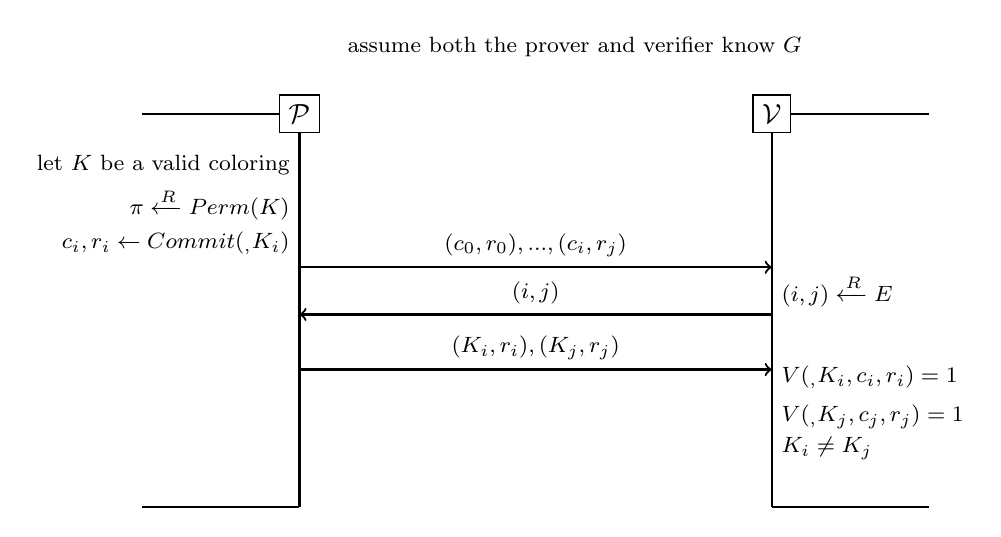
\begin{tikzpicture}
      \pause
        \node[draw] (Adversary) at (-3, 2) {\(\mathcal{P}\)}; 
        \draw[thick] (Adversary) -- ++(0, -5); 
        \draw[thick] (Adversary) -- ++(-2, 0);
        \draw[thick] (-3, -3) -- ++(-2, 0);

      \pause
        \node[draw] (Challenger) at (3,2) {\(\mathcal{V}\)}; 
        \draw[thick] (Challenger) -- ++(0, -5);
        \draw[thick] (Challenger) -- ++(2, 0);
        \draw[thick] (3, -3) -- ++(2, 0);

      \pause
        \node[draw=none,fill=none,anchor=east, font=\footnotesize] (choice0) at ($(Adversary) + (6.5,.85)$) {assume both the prover and verifier know \(G\)};

      \pause
        \node[draw=none,fill=none,anchor=east, font=\footnotesize] (choice0) at ($(Adversary) + (0,-.65)$) {let \(K\) be a valid coloring};
        \node[draw=none,fill=none,anchor=east, font=\footnotesize] (choice0) at ($(Adversary) + (0,-1.15)$) {\(\pi \xleftarrow[]{R} Perm(K)\)};
        \node[draw=none,fill=none,anchor=east, font=\footnotesize] (choice0) at ($(Adversary) + (0,-1.65)$) {\(c_i, r_i \leftarrow Commit(_, K_i)\)};
      \pause
        \draw[->,thick] ($(Adversary)+(0,-1.95)$) -- ($(Challenger)+(0,-1.95)$) node [pos=0.5,above,font=\footnotesize] {\((c_0, r_0),...,(c_i,r_j)\)};
      \pause
        \node[draw=none,fill=none,anchor=west, font=\footnotesize] (bit) at ($(Challenger) + (0,-2.25)$) {\((i,j) \xleftarrow[]{R} E \)};
      \pause
        \draw[->,thick] ($(Challenger)+(0,-2.55)$) -- ($(Adversary)+(0,-2.55)$) node [pos=0.5,above,font=\footnotesize] {\((i,j) \)};
      \pause
        \draw[->,thick] ($(Adversary)+(0,-3.25)$) -- ($(Challenger)+(0,-3.25)$) node [pos=0.5,above,font=\footnotesize] {\((K_i, r_i), (K_j, r_j)\)};
      \pause
        \node[draw=none,fill=none,anchor=west, font=\footnotesize] (bit) at ($(Challenger) + (0,-3.35)$) {\(V(_,K_i, c_i, r_i) = 1\)};
        \node[draw=none,fill=none,anchor=west, font=\footnotesize] (bit) at ($(Challenger) + (0,-3.85)$) {\(V(_, K_j, c_j, r_j) = 1\)};
        \node[draw=none,fill=none,anchor=west, font=\footnotesize] (bit) at ($(Challenger) + (0,-4.25)$) {\(K_i \neq K_j\)};
      \end{tikzpicture}
\end{frame}

\begin{frame}{Schnorr Signatures}
    \begin{itemize}
        \item \pause Verification Key is \((g, g^x)\)
        \item \pause To sign use a non-interactive zero knowledge proof of discrete log of \(x\) where the challenge \(c\) is derived from the message using a hash function
        \item \pause We use something very similar to this in practice called DSA/ECDSA
    \end{itemize}
\end{frame}

\begin{frame}{Failed Implementations}
    \begin{itemize}
        \item \pause For playstation 3 updates (and some bitcoin wallets), the updates are signed using schnorr signatures.
        \item \pause If the randomness of the constant \(r\) is not very good, then the signature isn't very secure
        \item \pause Some systems use fixed constants for the randomness and this allows hackers to deploy arbitrary firmware and other updates/signed messages!
        \item \pause lesson: avoid randomness reuse
    \end{itemize}
    
\end{frame}

\end{document}